\myframe{
  \ctr{Linguagens}

  \pause
  \begin{minipage}{0.6\textwidth}
    \begin{center}
      Fortran \qquad C \\
      MatLab \\ \vspace{0.7cm}
      \onslide<3->{
      Python \qquad Ruby \qquad Perl \\
      PHP \qquad Java \qquad Javascript \\
      C++ \qquad Shell \qquad Objective C \\
      C\# \qquad Assembly \qquad SQL \qquad R \\
      Makefile \qquad HTML \qquad Markdown
      }
    \end{center}
  \end{minipage}
  \begin{minipage}{0.35\textwidth}
    \begin{flushleft}
      Velocidade \\
      Praticidade \\ \vspace{0.7cm}
      \onslide<3->{
      Fazer um site; \\
      Parsear texto; \\
      Criar interfaces gráficas; \\
      Criar apps; \\
      Automatizar testes;
      }
    \end{flushleft}
  \end{minipage}
}

\myframe{
  \ctr{Julia}
  ``... a {\bf high-level}, {\bf high-performance} dynamic programming language
  for technical computing, with {\bf syntax that is familiar} to users of other
  technical computing environments. ''
  \pause
  \begin{itemize}
    \item<2-> Usa C e Fortran no código;
    \item<3-> Substitui o MatLab;
    \item<4-> Compatibilidade com C e Fortran;
    \item<5-> Velocidade.
  \end{itemize}
}

\myframe{
  \ctr{JuliaOpt}
  \begin{minipage}{0.2\textwidth}
    \includegraphics[scale=0.2]{assets/juliaopt.png}
  \end{minipage}
  \begin{minipage}{0.75\textwidth}
    \begin{itemize}
      \item Interfaces para alguns algoritmos conhecidos: IPOPT, CPLEX, KNITRO,
        COIN Cbc e Clp, entre outros.
      \item Linguagens de modelagem {\tt JuMP} e {\tt Convex}.
      \item Implementações de softwares tradicionais de otimização puramente em
        Julia.
    \end{itemize}
  \end{minipage}
}

\myframe{
  \ctr{Editores e IDEs}
  \begin{itemize}
    \item Vim (Vi)
    \item Emacs
    \item Atom
    \item Sublime text
    \item Eclipse
    \item Sharelatex e/ou Writelatex
  \end{itemize}
}

\myframe{
  \ctr{Eu}
  \begin{itemize}
    \item uso Vim com GNU Screen.
    \item Divido a tela em 2: um lado com o shell pra compilar e o outro para
      edição.
    \item Para LaTeX, deixo um lado com o PDF. Num dos screens, uso o
      {\tt latexmk} rodando continuamente.
  \end{itemize}
}

\lstset{
  basicstyle=\tt\tiny,
  breaklines=true,
  frame=single
}

\begin{frame}[t,fragile]
  \ctr{Perprof-py}
  \lstinputlisting{assets/alpha.table}
  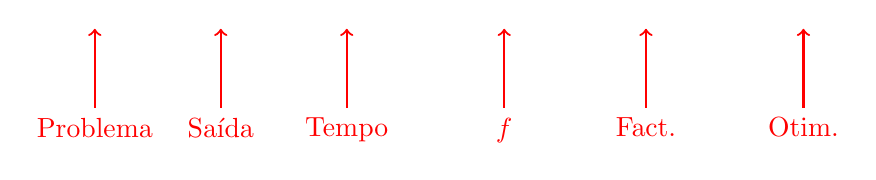
\begin{tikzpicture}
    \draw[thick,red,<-] (0.0,0) -- (0.0,-1) node[below] {Problema};
    \draw[thick,red,<-] (1.6,0) -- (1.6,-1) node[below] {Saída};
    \draw[thick,red,<-] (3.2,0) -- (3.2,-1) node[below] {Tempo};
    \draw[thick,red,<-] (5.2,0) -- (5.2,-1) node[below] {$f$};
    \draw[thick,red,<-] (7.0,0) -- (7.0,-1) node[below] {Fact.};
    \draw[thick,red,<-] (9.0,0) -- (9.0,-1) node[below] {Otim.};
  \end{tikzpicture}
\end{frame}

\myframetop{
  \ctr{Perprof-py}
  \begin{center}
    \only<1>{
      \includegraphics[height=0.6\textheight]{assets/abc-tikz.png} \\
      {\scriptsize \tt perprof-py *.table \ddash tikz -o abc}
    }
    \only<2>{
      \includegraphics[height=0.6\textheight]{assets/abc-semilog-tikz.png} \\
      {\scriptsize \tt perprof-py *.table \ddash semilog \ddash tikz -o abc-semilog}
    }
    \only<3>{
      \includegraphics[height=0.6\textheight]{assets/abc-semilog-bw-tikz.png} \\
      {\scriptsize \tt perprof-py *.table \ddash semilog \ddash tikz \ddash semilog
      \ddash black-and-white -o abc-bw}
    }
    \only<4>{
      \includegraphics[height=0.6\textheight]{assets/abc-100-tikz.png} \\
      {\scriptsize \tt perprof-py *.table \ddash semilog \ddash tikz \ddash
        semilog \ddash tau 100
      -o abc-100}
    }
    \only<5>{
      \includegraphics[height=0.6\textheight]{assets/abc-semilog-hs-tikz.png} \\
      {\scriptsize \tt perprof-py *.table \ddash semilog \ddash tikz \ddash semilog
      \ddash subset hs.subset -o abc-hs}
    }
  \end{center}
}

\myframe{
  \ctr{Git}
  \begin{center}
    \includegraphics[height=0.7\textheight]{assets/phd.png}
  \end{center}
}

\myframe{
  \ctr{Git}
  \begin{center}
    \includegraphics[height=0.5\textheight]{assets/version1.png}
    \hspace{0.1cm}
    \pause
    \includegraphics[height=0.5\textheight]{assets/version2.png}
    \hspace{0.1cm}
    \pause
    \includegraphics[height=0.5\textheight]{assets/version3.png}
    \hspace{0.1cm}
    \pause
    \includegraphics[height=0.5\textheight]{assets/version4.png}
    \hspace{0.1cm}
    \pause
    \includegraphics[height=0.5\textheight]{assets/version5.png}
  \end{center}
}

\myframe{
  \ctr{Código aberto}
  \begin{itemize}
    \item GitHub
    \item Bitbucket
    \item Gitorious
  \end{itemize}
}

\tikzstyle{local}=[draw, rectangle]
\tikzstyle{remoto}=[draw, circle]

\myframe{
  \ctr{Git remoto - GitHub}
  \begin{center}
    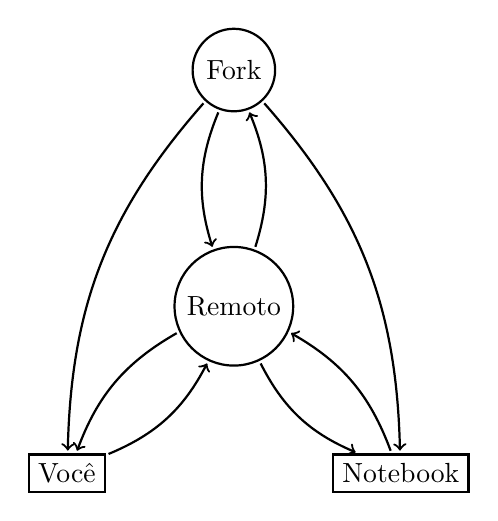
\begin{tikzpicture}[thick, node distance=3cm, bend angle=20, shorten <=1pt,
      shorten >=1pt, bend right]
      \node[local] (voce)   {Você};
      \onslide<2->{
        \node[remoto] (remote) [above right of=voce] {Remoto};
        \draw[->] (voce) to (remote);
      }
      \onslide<4->{
        \draw[->] (remote) to (voce);
      }
      \onslide<3->{
        \node[local] (note) [below right of=remote] {Notebook};
        \draw[->] (note) to (remote);
        \draw[->] (remote) to (note);
      }
      \onslide<5->{
        \node[remoto] (fork) [above of=remote] {Fork};
        \draw[->] (remote) to (fork);
      }
      \onslide<6->{
        \draw[->] (fork) to (remote);
        \draw[->] (fork) to (voce);
        \draw[->, bend left] (fork) to (note);
      }

    \end{tikzpicture}
  \end{center}
}

\myframe{
  \ctr{Github}
  \begin{itemize}
    \item {\bf Travis CI} \\
      Testes automatizados que começam quando você sobe o
      trabalho pro GitHub.
    \item {\bf Coveralls.io} \\
      De acordo com seus testes, ele verifica qual porcentagem
      do seu trabalho (em linhas úteis) está sendo verificada.
    \item {\bf GitHub Pages} \\
      Armazenamento de páginas estáticas, no formato
      {\tt http://usuario.github.io}.
  \end{itemize}
}

\myframe{
  \ctr{\LaTeX: TikZ e PgfPlots}
  \begin{itemize}
    \item {\bf PGF} ({\bf P}ortable {\bf G}raphics {\bf F}ormat)
      é uma camada básica, com comandos básicos.
    \item {\bf TikZ} ({\bf T}ikZ {\bf i}st {\bf k}ein
      {\bf Z}eichenprogramm - TikZ não é um programa para
      desenhar). Uma camada {\it frontend} com comandos facilitando
      o desenho utilizando PGF.
    \item {\bf PgfPlots} Faz gráficos de alta qualidade usando o
      TikZ. O usuário passa informações de eixo, e funções/dados.
  \end{itemize}
}

\myframe{
  \ctr{TikZ}
  \begin{center}
  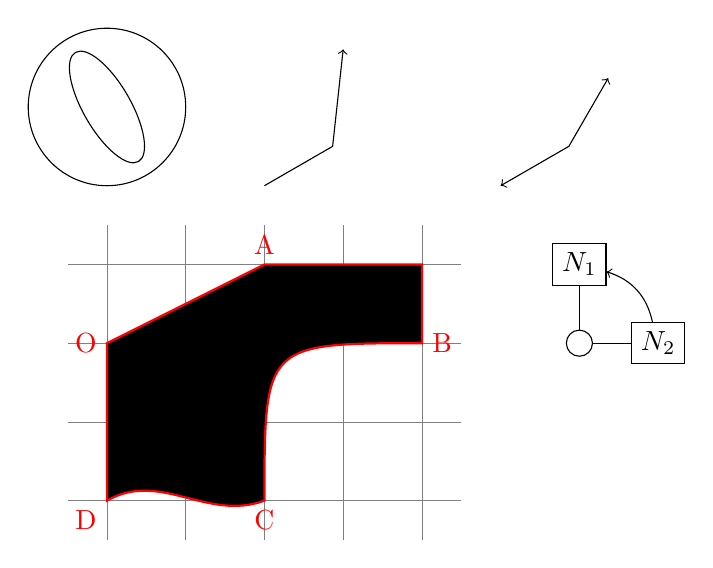
\begin{tikzpicture}
    \path[draw,->] (0,0) -- (30:1cm) -- (60:2cm);
    \draw[<->] (3,0) -- ++(30:1cm) -- ++(60:1cm);
    \draw[help lines, shift={(-2,-2)}] (-0.5,-2.5) grid (4.5,1.5);
    \path[fill,draw=red,fill=black,thick,shift={(-2,-2)}]
      (0,0) node[left,red] {O} -- (2,1) node[above,red] {A}
                          -| (4,0) node[right,red] {B}
                          .. controls (2,0) .. (2,-2) node[below,red] {C}
                          to[out=200,in=30] (0,-2) node[below left, red] {D}
                          -- cycle;
    \draw (-2,1) circle[radius=1];
    \draw (-2,1) circle[x radius=0.3, y radius=0.8, rotate=30];
    \node[draw,rectangle,black] (p1) at (4,-1) {$N_1$};
    \coordinate[draw,circle] (p2) at (4,-2);
    \node[draw,rectangle,black] (p3) at (5,-2) {$N_2$};
    \draw (p1) -- (p2) -- (p3);
    \draw[->] (p3) to[bend right] (p1);
  \end{tikzpicture}
  \end{center}
}

\begin{frame}
  \begin{center}
    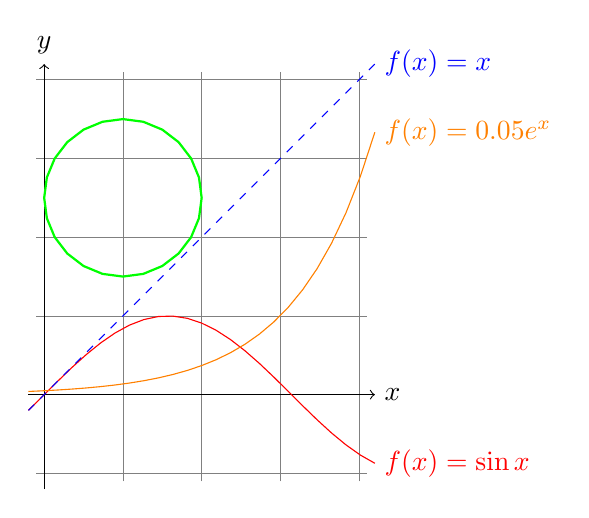
\begin{tikzpicture}[domain=-0.2:4.2]
    \draw[very thin,gray] (-0.1,-1.1) grid (4.1,4.1);
    \draw[->] (-0.2,0) -- (4.2,0) node[right] {$x$};
    \draw[->] (0,-1.2) -- (0,4.2) node[above] {$y$};
    \draw[red]  plot(\x,{sin(\x r)}) node[right] {$f(x)=\sin x$};
    \draw[blue,dashed] plot(\x,\x) node[right] {$f(x)=x$};
    \draw[orange] plot(\x,{0.05*exp(\x)}) node[right] {$f(x)=0.05e^x$};
    \draw[green,thick,domain=0:360]  plot({1+cos(\x)},{2.5+sin(\x)});
  \end{tikzpicture}
  \end{center}
\end{frame}

\begin{frame}
  \begin{center}
    \begin{tikzpicture}[scale=2]
    \draw[->] (-0.1,0) -- (2.1,0);
    \draw[->] (0,-0.1) -- (0,1.8);
    \draw[domain=0:1.75,red] plot (\x,{0.5*\x^2});
    \foreach \x in {0.5, 0.75, ..., 1.25} {
      \draw (\x,0) -- (\x,{0.5*\x^2}) -- ({\x+0.25},{0.5*\x^2}) -- ({\x+0.25},0)
      -- cycle;
    }
    \draw[blue] (0.5,0.125) -- (0.5,0) node[below] {$a$};
    \draw[blue] (1.5,1.125) -- (1.5,0) node[below] {$b$};
  \end{tikzpicture}
  \end{center}
\end{frame}

\myframe{
  \ctr{PgfPlots}
  \begin{center}
    \only<1>{
      \includegraphics[height=0.75\textheight]{assets/pgfplots-ex1.pdf}
    }
    \only<2>{
      \includegraphics[height=0.75\textheight]{assets/pgfplots-ex2.pdf}
    }
    \only<3>{
      \includegraphics[height=0.75\textheight]{assets/pgfplots-ex3.pdf}
    }
    \only<4>{
      \includegraphics[height=0.75\textheight]{assets/filtro.pdf}
    }
    \only<5>{
      \includegraphics[height=0.75\textheight]{assets/filtro-fh.pdf}
    }
    \only<6>{
      \includegraphics[height=0.75\textheight]{assets/mountain.pdf}
    }
    \only<7>{
      \includegraphics[height=0.75\textheight]{assets/mountain-cm.pdf}
    }
  \end{center}
}
